\documentclass[tikz, border=5pt]{standalone}
\usetikzlibrary{arrows.meta, positioning, calc}

\begin{document}
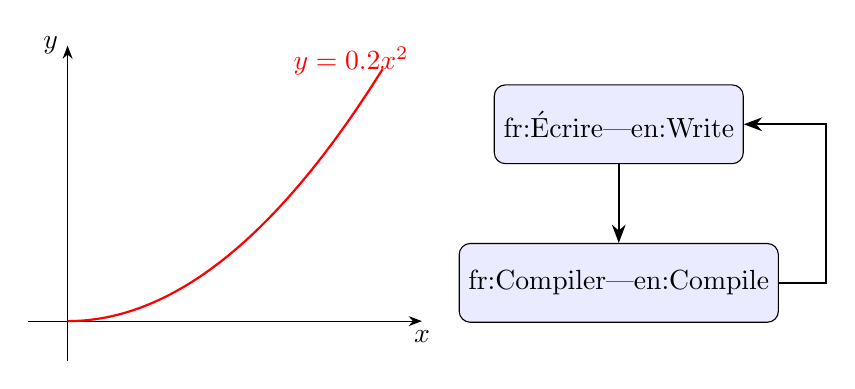
\begin{tikzpicture}[
    >=Stealth,
    box/.style={draw, rounded corners, fill=blue!8, minimum width=2.6cm, minimum height=1cm, align=center},
  ]
  % {{fr:Axes|en:Axes}}
  \draw[->] (-0.5,0) -- (4.5,0) node[below] {$x$};
  \draw[->] (0,-0.5) -- (0,3.5) node[left] {$y$};
  % {{fr:Courbe|en:Curve}}
  \draw[thick, red, domain=0:4, smooth, samples=50] plot (\x, {0.2*\x*\x});
  \node[red] at (3.6,3.3) {$y = 0.2x^2$};
  % {{fr:Schéma|en:Diagram}}
  \node[box] (a) at (7,2.5) {{{fr:Écrire|en:Write}}};
  \node[box, below=of a] (b) {{{fr:Compiler|en:Compile}}};
  \draw[->, thick] (a) -- (b);
  \draw[->, thick] (b.east) -- ++(0.6,0) |- (a.east);
\end{tikzpicture}
\end{document}
